\documentclass[conference]{IEEEtran}

\usepackage[T1]{fontenc}
\usepackage[utf8]{inputenc}
\usepackage{graphicx}
\usepackage{booktabs}
\usepackage{tabularx}
\usepackage{array}
\usepackage{multirow}
\usepackage{microtype}
\usepackage{balance}
\usepackage{url}
\usepackage[hidelinks]{hyperref}

\newcolumntype{Y}{>{\raggedright\arraybackslash}X}
\newcommand{\absTau}{|\tau|}

\title{Group 10: Robustness Boundaries of Learning-to-Rank LLM Scheduling\\
{\large A Case Study of vLLM-LTR under Distribution Shift}}

\author{
\IEEEauthorblockN{Yuze Gao, Yuh Jen Sun, Shun Huang, Chenxi Li, and Mengze Hu}
\IEEEauthorblockA{FDU MSACS Capstone, CSCI 6806 / INFO 4205\\
July 2026}
}

\begin{document}
\maketitle

\begin{abstract}
Learning-to-rank (LTR) scheduling reduces head-of-line blocking by predicting output behavior and admitting shorter requests first. We reproduce vLLM-LTR on one RTX 3090 and confirm an 8.1$\times$ reduction in mean time to first token (TTFT) under matched LMSYS traffic.

Under LMSYS-to-ShareGPT distribution shift, ranking quality and tail latency degrade, and raw LTR can exhaust swap space. A waiting-time aging gate with preemption protection restores 500/500 completion at the stressed rate while retaining lower mean TTFT than FCFS. The results show that early, memory-aware guardrails are necessary when learned admission scores are deployed.
\end{abstract}

\section{Introduction}
Interactive LLM serving is dominated by queueing effects. Under load, a long request at the head of a first-come, first-served (FCFS) queue delays shorter requests behind it. vLLM-LTR \cite{fu2024ltr} ranks waiting requests with a small learned predictor of output length and therefore approximates shortest-job-first scheduling. This design can sharply reduce average waiting time and TTFT.

The unresolved deployment question is whether a predictor trained on one request distribution remains useful when prompts, applications, or user behavior change. This question matters because a ranking error is not only a statistical error: after admission, it changes batching, KV-cache occupancy, and preemption behavior in the serving engine \cite{kwon2023pagedattention}.

Our project began as a reproduction of the NeurIPS 2024 scheduler and developed into a boundary study. We evaluate matched LMSYS traffic \cite{zheng2024lmsys}, a ShareGPT-based distribution shift \cite{sharegpt2023}, and a minimal guarded scheduler. We distinguish ranking quality, mean latency, tail latency, and availability so that a fast partial run is never reported as a successful serving result.

The work makes three contributions:
\begin{itemize}
    \item \textbf{Reproduction and characterization.} We reproduce the in-distribution benefit and identify ranking degradation, tail-latency inversion, and an engine crash under shift.
    \item \textbf{Mechanism and mitigation.} We connect mis-ranking to bounded swap-mode preemption and evaluate an aging gate with preemption protection.
    \item \textbf{Ablation and reproducibility.} We separate predictor quality from decision timing and maintain pinned environments, manifests, raw logs, and code-generated figures.
\end{itemize}

\section{Background}
\subsection{vLLM Memory Mechanics}
vLLM uses continuous batching and PagedAttention to manage a paged KV cache \cite{kwon2023pagedattention}. Each running request holds GPU memory proportional to its context. In the studied fork, preempted KV pages are moved to a bounded CPU swap pool. With \texttt{--swap-space 4}, the pool is limited to 4 GB. If a new preemption cannot be accommodated, the engine aborts. Fig.~\ref{fig:architecture} summarizes the resulting admission and memory-allocation path.

\begin{figure}[t]
    \centering
    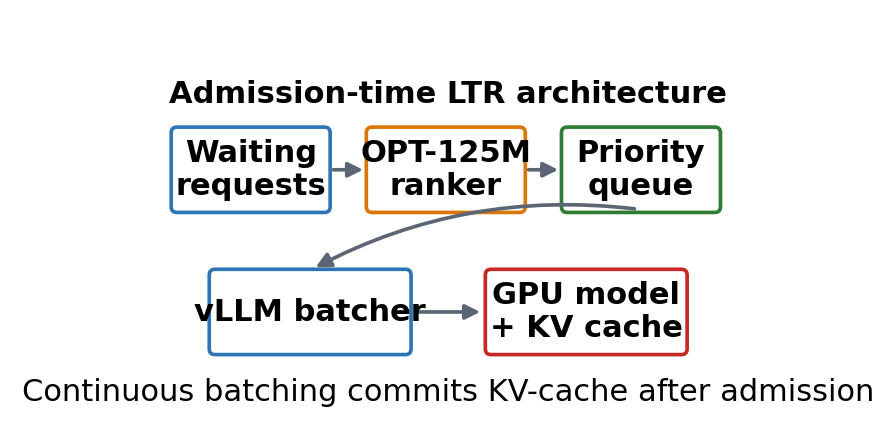
\includegraphics[width=\columnwidth]{figures/background_architecture.png}
    \caption{System architecture of the reproduced admission-time LTR scheduler.}
    \label{fig:architecture}
\end{figure}

As shown in Fig.~\ref{fig:architecture}, the serving path has two timing regimes. The predictor must act before prefill to change which request enters the batch; signals computed from the main model after prefill can improve score quality but cannot undo the memory already committed to that request. This timing distinction becomes central in the later attribution study.

TTFT contains both queueing delay and prompt-prefill time, whereas time per output token is measured during autoregressive decoding. Admission order primarily changes the queueing component, but the requests selected together also determine how much KV state must coexist on the GPU. Consequently, two policies with similar average predictor error can produce different memory pressure and tail latency once continuous batching is active.

\subsection{FCFS and Learning-to-Rank Admission}
FCFS preserves arrival order but suffers head-of-line blocking. vLLM-LTR instead uses an OPT-125M ranker \cite{zhang2022opt} trained with a ListMLE loss on prompt and output-length pairs from LMSYS \cite{zheng2024lmsys}. The ranker scores requests before prefill, so its estimate is early enough to affect admission. The benefit depends on the training and serving distributions remaining similar. Fig.~\ref{fig:failurepath} shows the memory-coupled components through which an incorrect early decision becomes a systems failure.

\begin{figure}[t]
    \centering
    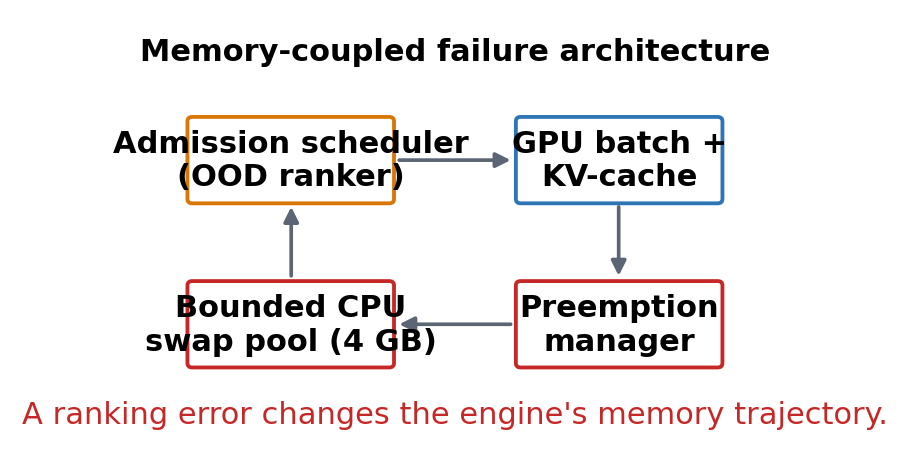
\includegraphics[width=\columnwidth]{figures/background_failure_path.png}
    \caption{Memory-coupled components that turn OOD mis-ranking into swap exhaustion.}
    \label{fig:failurepath}
\end{figure}

\subsection{Why Distribution Shift Is a Systems Problem}
A shifted workload can change output-length patterns without changing the serving API. Incorrect rankings admit memory-intensive requests too early, increase overlapping KV-cache demand, and trigger repeated preemptions. The feedback path in Fig.~\ref{fig:failurepath} explains why an apparently modest drop in Kendall ranking correlation can produce a large tail-latency or availability failure.

The failure is cumulative rather than request-local. One underestimated long generation remains in the batch for many decode steps, reducing the free-block budget for later arrivals. Additional requests can then be swapped or recomputed, and their renewed allocation attempts increase pressure again. The scheduler therefore changes a shared resource trajectory, not only the completion order of one pair of requests.

\subsection{Deployment Properties}
A deployable scheduler must satisfy more than low mean latency. It should bound starvation, preserve service for urgent short requests, avoid preemption cascades, and fall back toward arrival order when predictions are unreliable. These properties motivate the aging and preemption controls used in our guarded policy.

Waiting-time aging and preemption protection address separate risks. Aging gradually reduces the influence of a stale learned score, which prevents requests from remaining behind newly arriving work indefinitely. Protection acts after admission by preserving running work when the next batch is formed. Neither mechanism requires the scheduler to know the true output length, and both retain FCFS as a conservative reference point.

\subsection{Fixed Experimental Environment}
All hardware claims use one NVIDIA RTX 3090 (24 GB), Meta-Llama-3-8B-Instruct \cite{dubey2024llama3}, the \texttt{vllm-ltr} fork at commit \texttt{13bbf6ff}, vLLM 0.4.1, PyTorch 2.2.1+cu121 \cite{paszke2019pytorch}, and 500 prompts per arm. Simulation results are explicitly labeled and are not treated as hardware measurements.

\subsection{Measurement Interpretation}
Mean TTFT measures the average interactive response, p99 exposes the worst queueing behavior, and completion count records whether a policy remains available. Offline Kendall correlation is used only to diagnose ordering quality. It cannot establish deployment safety by itself because it does not include batching, KV-cache allocation, or the finite swap pool.

\section{Related Work}
\subsection{Serving and Memory Management}
PagedAttention and continuous batching made KV-cache management a first-class serving concern \cite{kwon2023pagedattention}. SGLang reuses prefixes through RadixAttention \cite{zheng2024sglang}, PromptCache reuses attention states for repeated prompt segments \cite{gim2024promptcache}, Hydragen shares computation over common prefixes \cite{juravsky2024hydragen}, and Sarathi-Serve chunks prefill to reduce generation stalls \cite{agrawal2024sarathi}. These systems improve memory or compute reuse, but they do not directly establish that a learned admission order remains safe off distribution.

These mechanisms operate at different points in the request lifetime. Prefix reuse and chunked prefill reduce work after a prompt is known, while admission ranking decides which request receives resources first. Their benefits can be complementary, but a cache hit should not be interpreted as evidence that a request will generate few output tokens.

\subsection{Predictive and SLO-Aware Scheduling}
vLLM-LTR \cite{fu2024ltr} provides the closest baseline because it changes request order using predicted output behavior. Its strength is large TTFT reduction when the predictor matches the workload; its limitation is reliance on a fixed predictor distribution. SLO-aware scheduling \cite{huang2025slo} adds task-level deadlines and service objectives to priority. Apt-Serve \cite{gao2025aptserve} adapts batch composition and hybrid-cache allocation to runtime state. Both papers motivate guardrails beyond a single predicted length.

SLO-aware priority asks whether a request is close to violating a service target, whereas Apt-Serve asks whether the current cache and batch state can support a different composition. Both are runtime signals rather than replacements for output-length prediction. Our related-work probes therefore treat them as candidate constraints around LTR, not as directly comparable latency measurements.

\subsection{Position of This Study}
Our study does not propose another unguarded ranking score. Instead, it tests the deployment boundary of an existing learned scheduler and asks which controls prevent a statistical error from becoming an availability failure. Early simulation probes of SLO-aware and hybrid-cache priority were used only as related-work probes; the central claims in this report come from vLLM hardware runs.

This distinction also determines the evidence hierarchy in the report. Offline probes are useful for rejecting weak signals, simulation explores policy behavior cheaply, and the final availability claims require the CUDA serving engine. A result is cited only at the level supported by the system that produced it.

\subsection{Prefix-Cache Signals}
Prefix reuse is valuable for prefill and memory efficiency, but it is not equivalent to predicting output length. Our offline probe observes reuse opportunities yet finds no measurable improvement in output-length rank correlation when a cache bonus is added. The result supports treating cache state as a complementary serving signal rather than a replacement for admission-time prediction.

\subsection{Research Gap}
Recent systems separately optimize ranking, service objectives, cache reuse, and batch formation. The missing link is a hardware evaluation of what happens when a learned admission score is wrong and memory pressure amplifies that error. Our work fills this narrower gap by measuring the failure boundary and testing minimal controls in the same vLLM-LTR code path.

\subsection{Queueing Safeguards and Fallback Policies}
Shortest-job-first policies reduce average waiting time when service estimates are accurate, but they require an explicit fairness mechanism when estimates are stale. FCFS supplies a useful fallback because its ordering does not depend on predictor calibration. SLO-aware scheduling \cite{huang2025slo} adds urgency through deadlines, while our aging gate adds urgency through observed queue residence time. The two controls are related but not interchangeable: a deadline expresses an application objective, whereas aging protects any request from indefinite displacement.

Preemption introduces a second control point. Reordering waiting work changes admission, but evicting an already running request changes memory occupancy and discards or transfers useful state. A policy can therefore be fair at the queue and still be unstable after admission. This distinction motivates evaluating aging together with preemption protection rather than treating queue priority as the complete scheduler.

\subsection{Comparison Boundary}
The related systems use different models, traces, memory budgets, and definitions of success, so their headline speedups are not combined into one numerical ranking. We compare mechanisms instead: vLLM-LTR supplies an early learned score \cite{fu2024ltr}, SLO-aware scheduling supplies task urgency \cite{huang2025slo}, Apt-Serve supplies runtime cache and batch awareness \cite{gao2025aptserve}, and prefix-serving systems supply reuse signals \cite{zheng2024sglang,gim2024promptcache,juravsky2024hydragen,agrawal2024sarathi}. The hardware experiments then ask which of these signal types can be acted on early enough to protect the reproduced vLLM-LTR serving path.

This scope also prevents simulation outcomes from being reported as GPU measurements. Simulation is used to test policy logic and reject weak ideas before an expensive run; the CUDA experiments are used for latency, completion, and failure claims. Keeping those levels separate makes the comparison reproducible and avoids attributing a synthetic latency model to the real serving engine.

\section{Methodology}
\subsection{Reproducible Environment}
\begin{table}[t]
\caption{Fixed Hardware and Software Environment}
\label{tab:environment}
\centering
\footnotesize
\begin{tabularx}{\columnwidth}{@{}lY@{}}
\toprule
\textbf{Component} & \textbf{Pinned value} \\
\midrule
GPU & NVIDIA RTX 3090, 24 GB \\
Model & Meta-Llama-3-8B-Instruct \\
Serving stack & \texttt{vllm-ltr} @ \texttt{13bbf6ff}; vLLM 0.4.1 \\
Framework & PyTorch 2.2.1+cu121 \\
Memory & 4 GB CPU swap; swap-mode preemption \\
Load & 500 prompts; Poisson arrivals, 2--32 req/s \\
Paper predictor & OPT-125M, ListMLE, LMSYS training \\
\bottomrule
\end{tabularx}
\end{table}

Table~\ref{tab:environment} fixes the hardware and software boundary for all serving claims; changing any of these values defines a different experimental environment.

\subsection{Workload Provenance}
The matched LMSYS workload is taken from the public Llama3-Trace artifact \cite{llmltr2024trace}. ShareGPT \cite{sharegpt2023} is used as the shifted conversation source, while Alpaca \cite{taori2023alpaca} appears only in the predictor ablation. Train and test provenance is recorded separately for every phase. Table~\ref{tab:provenance} makes the train-test relation explicit so that matched-distribution stability is not presented as OOD evidence.

\begin{table}[t]
\caption{Experimental Provenance; Phase D Is Not OOD Evidence}
\label{tab:provenance}
\centering
\footnotesize
\begin{tabular}{@{}llllc@{}}
\toprule
\textbf{Experiment} & \textbf{Train} & \textbf{Test} & \textbf{Relation} & \textbf{Seeds} \\
\midrule
ID sweep & LMSYS & LMSYS & Matched & 0 \\
OOD characterization & LMSYS & ShareGPT & OOD & 0 \\
Phase A/C mitigation & LMSYS & ShareGPT & OOD & 0 \\
Phase D stability & ShareGPT & ShareGPT & Matched & 0--2 \\
\bottomrule
\end{tabular}
\end{table}

\subsection{Metrics and Validity Rules}
Table~\ref{tab:metrics} defines the metrics and the reporting rules applied before aggregation.

\begin{table}[t]
\caption{Metrics and Validity Rules}
\label{tab:metrics}
\centering
\footnotesize
\begin{tabularx}{\columnwidth}{@{}lYY@{}}
\toprule
\textbf{Metric} & \textbf{Purpose} & \textbf{Reporting rule} \\
\midrule
Mean TTFT & Average queueing response & Seconds; completed arms only \\
p99 TTFT / latency & Tail behavior & Label the latency definition \\
Completion & Availability & Completed / 500 \\
$\absTau$ & Offline rank quality & Absolute value; dataset named \\
\bottomrule
\end{tabularx}
\end{table}

A crashed arm is reported by completion count and failure mechanism; its partial latency samples are excluded from aggregate comparisons. Every retained result is associated with a run manifest and SHA-256 identifier so that generated figures can be traced back to a specific data version.

\subsection{Model-Internal Predictor Ablation}
We train small ranking heads on Llama-3-8B hidden states captured after prefill: entropy-weighted pooling, mean pooling, and the last-token state. A two-layer MLP and a ridge floor are evaluated on held-out LMSYS, ShareGPT, and Alpaca \cite{taori2023alpaca}. The ablation isolates feature quality, but these signals arrive after prefill and therefore cannot make the original admission decision.

Each head is evaluated with the same request identifiers and output-length labels as the external predictor so that only the feature source changes. We report absolute Kendall correlation because the scheduler uses relative order rather than calibrated token counts. The comparison is diagnostic: a better post-prefill rank does not imply that the feature can be moved earlier in the serving path.

\subsection{Guarded Scheduler}
The V1 mitigation keeps the original LTR score and adds two controls. A request waiting longer than $T$ is promoted toward FCFS-equivalent priority; $T$ is swept over 30, 60, and 120 s. Preemption protection prevents a newly admitted request from evicting work already running. V1 uses $T=60$ s with protection because it balances mean and tail latency while preventing swap exhaustion.

The gate is evaluated at admission time using the request's accumulated queue delay. Before the threshold, the original learned ordering is preserved; after the threshold, arrival age dominates the request's effective priority. Protection does not reserve a fixed GPU partition. It constrains the next scheduling choice so that already allocated requests are not repeatedly displaced by a new score. This keeps the intervention local to the scheduler.

\subsection{Artifact Protocol}
Scripts pin seeds and configurations, preserve crash logs separately, regenerate Matplotlib \cite{hunter2007matplotlib} figures from result manifests, and verify parsers and aggregation rules with automated tests. This separation prevents simulated probes, matched-distribution runs, and true OOD hardware runs from being cited as interchangeable evidence.

Every benchmark arm writes its model, predictor, workload, request rate, seed, completion count, and latency definition to a machine-readable result. Aggregation scripts reject incompatible arms and retain failed runs as availability evidence instead of silently dropping them. Figure generation reads these records directly; no reported value is manually transcribed into a plot.

\section{Evaluation}
\subsection{In-Distribution Reproduction}
Under LMSYS traffic matched to predictor training, LTR reproduces the expected benefit. At rate 8, mean TTFT falls from 16.362 s under FCFS to 2.026 s under LTR. The gain is load dependent: at rate 2 there is little queueing and predictor overhead outweighs reordering, while rates 4--32 benefit. Table~\ref{tab:id} reports the exact values; Figs.~\ref{fig:mean-ttft} and \ref{fig:speedup} show the load-dependent trend and speedup.

\begin{table}[t]
\caption{In-Distribution Mean TTFT (Seconds), 500 Requests per Arm}
\label{tab:id}
\centering
\footnotesize
\begin{tabular}{@{}rrrr@{}}
\toprule
\textbf{Rate} & \textbf{FCFS} & \textbf{LTR} & \textbf{Speedup} \\
\midrule
2  & 0.111  & 0.130 & 0.85$\times$ \\
4  & 1.122  & 0.234 & 4.8$\times$ \\
8  & 16.362 & 2.026 & 8.1$\times$ \\
16 & 18.457 & 2.915 & 6.3$\times$ \\
32 & 21.215 & 6.095 & 3.5$\times$ \\
\bottomrule
\end{tabular}
\end{table}

\begin{figure}[t]
    \centering
    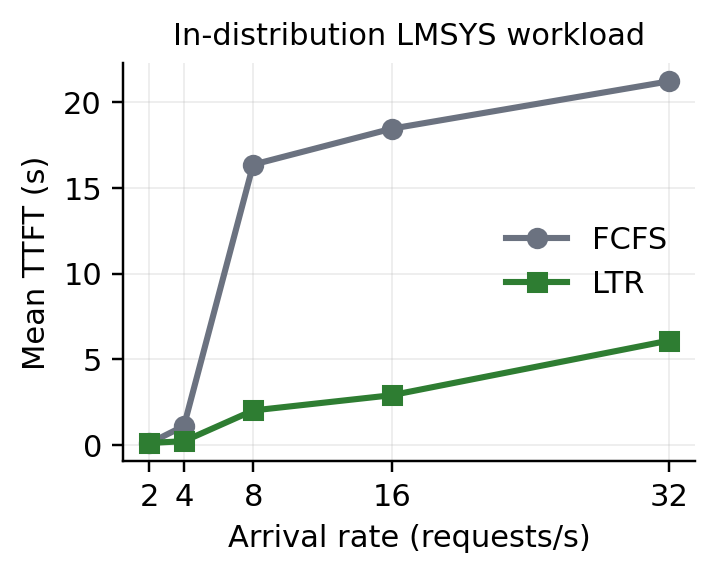
\includegraphics[width=0.97\columnwidth]{figures/eval_01_mean_ttft.png}
    \caption{Mean TTFT versus arrival rate under matched LMSYS traffic.}
    \label{fig:mean-ttft}
\end{figure}

\begin{figure}[t]
    \centering
    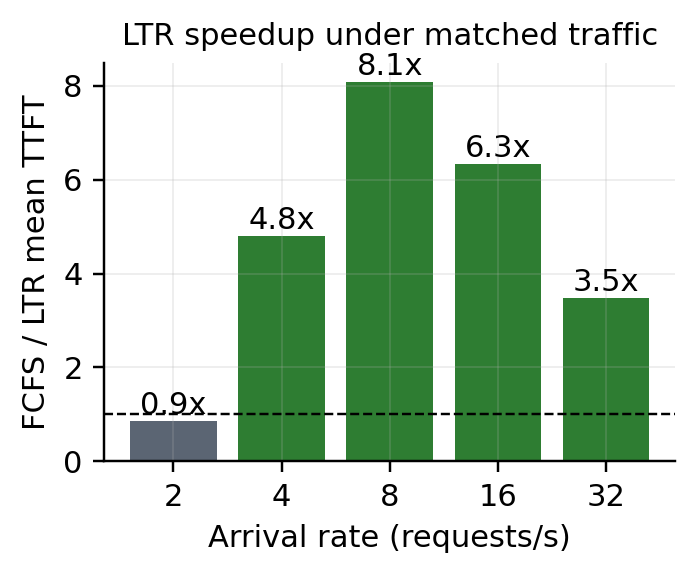
\includegraphics[width=0.97\columnwidth]{figures/eval_02_speedup.png}
    \caption{Mean-TTFT speedup from admission-time ranking.}
    \label{fig:speedup}
\end{figure}

\subsection{Distribution Shift Produces Three Failures}
Serving ShareGPT with the LMSYS-trained ranker produces a triple failure. Ranking quality drops from 0.642 to 0.420. At rate 4, raw LTR retains a lower mean TTFT but its p99 request latency rises to 230.981 s, compared with 150.170 s for FCFS. At rate 8, a preemption storm exhausts the 4 GB swap pool after only 15 completed requests, whereas FCFS completes all 500. Figs.~\ref{fig:tau-shift}--\ref{fig:completion} separate the offline rank degradation, tail inversion, and completion failure.

\begin{figure}[t]
    \centering
    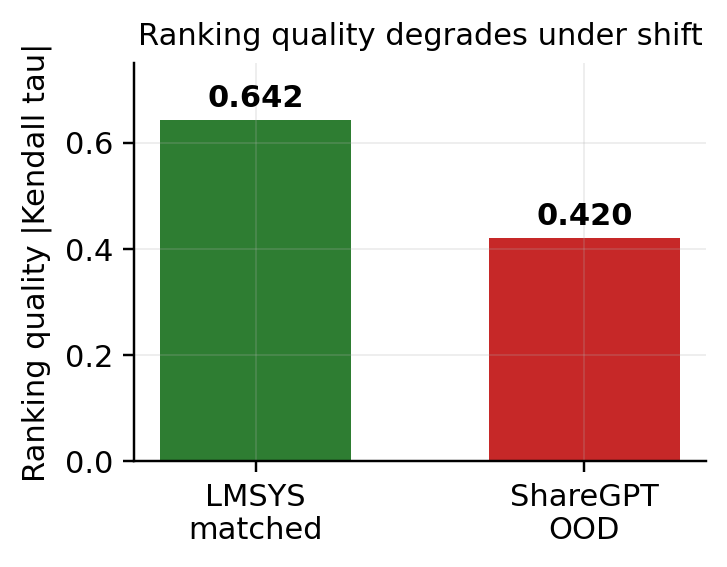
\includegraphics[width=0.97\columnwidth]{figures/eval_03_tau_shift.png}
    \caption{Offline ranking quality before and after distribution shift.}
    \label{fig:tau-shift}
\end{figure}

\begin{figure}[t]
    \centering
    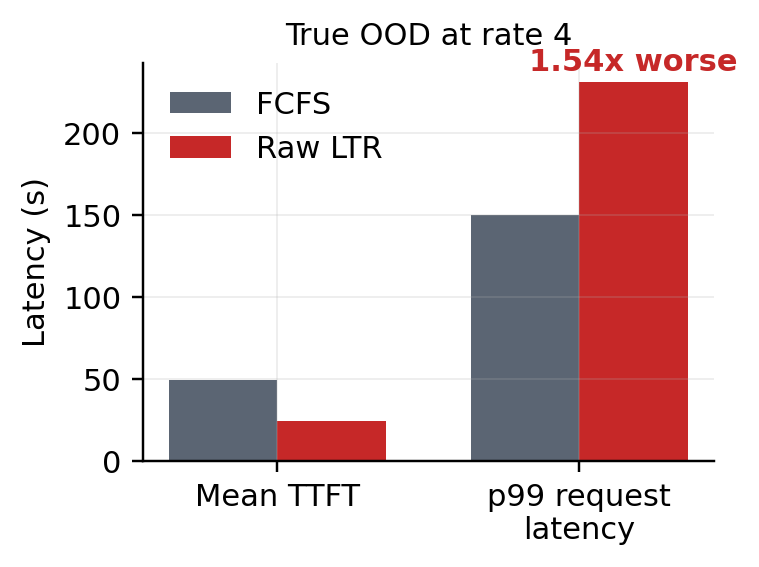
\includegraphics[width=0.97\columnwidth]{figures/eval_04_ood_tail.png}
    \caption{Tail-latency inversion under true OOD traffic at rate 4.}
    \label{fig:ood-tail}
\end{figure}

\begin{figure}[t]
    \centering
    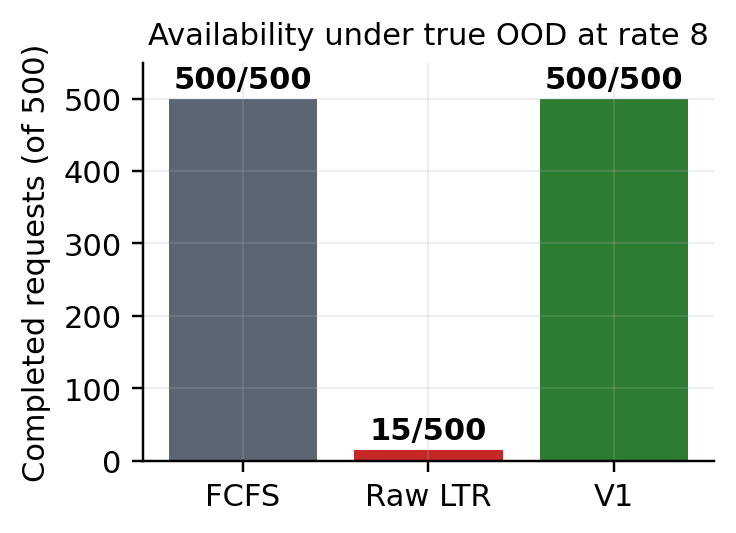
\includegraphics[width=0.97\columnwidth]{figures/eval_05_completion.png}
    \caption{Rate-8 completion counts expose the availability failure.}
    \label{fig:completion}
\end{figure}

\subsection{V1 Mitigation under True OOD Load}
Phase A/C keeps the predictor trained on LMSYS and serves ShareGPT. V1 is the only LTR-based arm that completes 500/500 at both tested rates. At rate 4, it improves mean TTFT over FCFS by 1.34$\times$ and also improves p99 TTFT. At rate 8, V1 survives and remains faster than FCFS, whereas raw LTR and aging-only policies crash. Table~\ref{tab:true-ood} provides the hardware measurements, while Fig.~\ref{fig:gate-threshold} shows why the 60 s threshold is selected rather than treating aging as a free parameter.

\begin{table}[t]
\caption{True OOD Hardware Results; Latencies Are TTFT in Seconds}
\label{tab:true-ood}
\centering
\scriptsize
\begin{tabular}{@{}llrrr@{}}
\toprule
\textbf{Rate} & \textbf{Policy} & \textbf{Done} & \textbf{Mean} & \textbf{p99} \\
\midrule
4 & FCFS & 500/500 & 49.599 & 110.355 \\
4 & Raw LTR & 500/500 & 24.254 & 156.162 \\
4 & Aging 120 + prot. & 500/500 & 27.355 & 120.292 \\
4 & V1: aging 60 + prot. & 500/500 & 37.070 & 97.951 \\
8 & FCFS & 500/500 & 69.287 & 158.930 \\
8 & Raw / aging-only & 15/500 & -- & -- \\
8 & V1: aging 60 + prot. & 500/500 & 61.038 & 147.871 \\
\bottomrule
\end{tabular}
\end{table}

\begin{figure}[t]
    \centering
    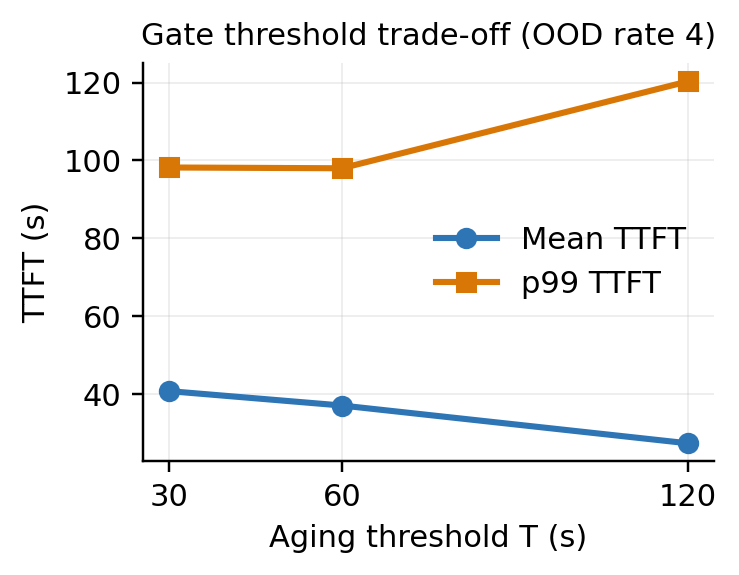
\includegraphics[width=0.97\columnwidth]{figures/eval_06_gate_threshold.png}
    \caption{Aging-threshold trade-off with protection enabled.}
    \label{fig:gate-threshold}
\end{figure}

\subsection{Multi-Seed Stability and Scope}
Phase D retrains the predictor on ShareGPT and evaluates ShareGPT, so it is a matched-distribution stability check rather than additional OOD evidence. Across seeds 0--2, V1 improves both mean and p99 TTFT over FCFS at rates 4 and 8. Raw LTR at rate 8 completes only under seed 1, showing that survival remains seed dependent even when the traffic distribution is matched. Table~\ref{tab:multiseed} and Fig.~\ref{fig:multiseed} summarize this three-seed check.

\begin{table}[t]
\caption{Matched ShareGPT Stability Check, Mean $\pm$ Std over Seeds 0--2}
\label{tab:multiseed}
\centering
\scriptsize
\begin{tabular}{@{}llrr@{}}
\toprule
\textbf{Rate} & \textbf{Policy} & \textbf{Mean TTFT} & \textbf{p99 TTFT} \\
\midrule
4 & FCFS & $40.438 \pm 2.082$ & $95.977 \pm 2.100$ \\
4 & Raw LTR & $22.873 \pm 1.228$ & $148.592 \pm 4.162$ \\
4 & V1 & $34.849 \pm 3.172$ & $87.653 \pm 6.375$ \\
8 & FCFS & $67.579 \pm 1.577$ & $153.551 \pm 3.149$ \\
8 & Raw LTR (seed 1) & 36.863 & 158.825 \\
8 & V1 & $59.764 \pm 1.165$ & $148.386 \pm 5.119$ \\
\bottomrule
\end{tabular}
\end{table}

\begin{figure}[t]
    \centering
    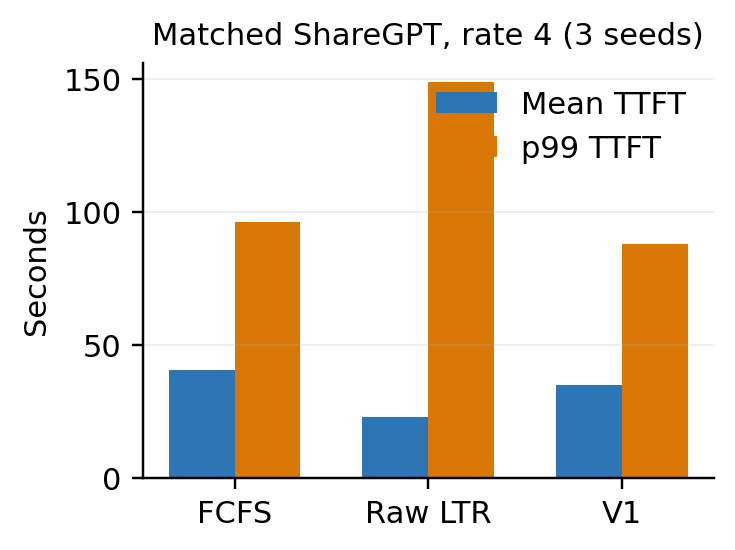
\includegraphics[width=0.97\columnwidth]{figures/eval_08_multiseed.png}
    \caption{Rate-4 matched-distribution stability check across three seeds.}
    \label{fig:multiseed}
\end{figure}

\subsection{Predictor and Timing Ablations}
The last-token MLP obtains the strongest LMSYS ranking quality (0.713) and slightly exceeds the OPT-125M baseline on ShareGPT (0.428 versus 0.420). Entropy-weighted pooling is weaker, so the motivating entropy hypothesis is not supported. More importantly, post-prefill scores arrive after KV-cache commitment; both post-prefill re-scoring policies still crash at rate 8. An oracle-quality admission score survives, indicating that information timing is at least as important as quality. Figs.~\ref{fig:predictor-ablation} and \ref{fig:attribution} distinguish predictor accuracy from decision timing.

\begin{figure}[t]
    \centering
    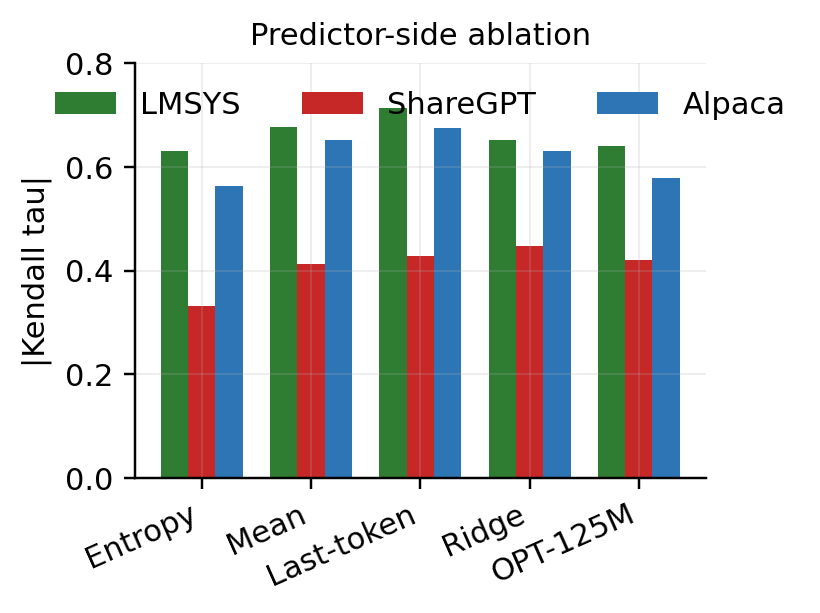
\includegraphics[width=0.97\columnwidth]{figures/eval_07_predictor_ablation.png}
    \caption{Predictor-side ranking ablation across three traces.}
    \label{fig:predictor-ablation}
\end{figure}

\begin{figure}[t]
    \centering
    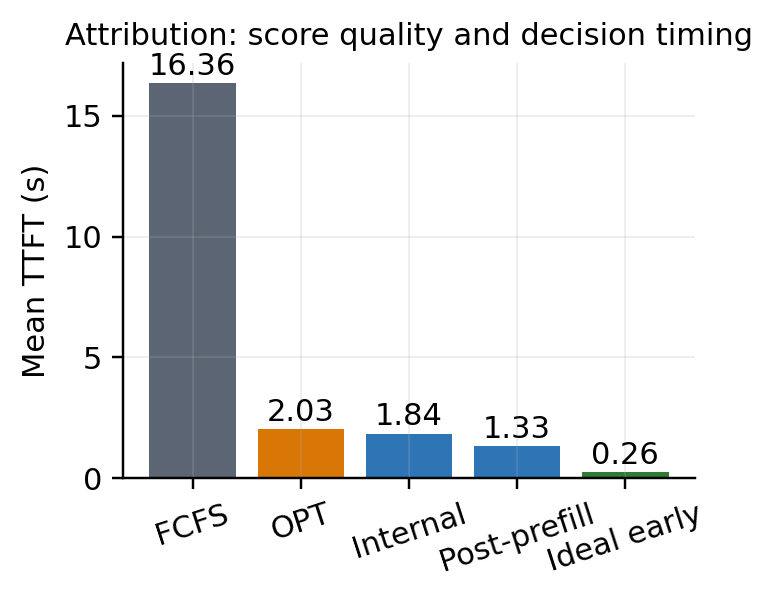
\includegraphics[width=0.97\columnwidth]{figures/eval_09_attribution.png}
    \caption{Attribution separates predictor quality from admission-time availability.}
    \label{fig:attribution}
\end{figure}

\subsection{Negative Results}
Zero-training entropy features did not provide a reliable ranker, and the cache-prefix probe did not improve output-length correlation. Post-prefill re-scoring improved simulated mean TTFT but did not prevent the rate-8 crash. We retain these results because they rule out attractive but mistimed signals and narrow the design space for the guarded scheduler.

\subsection{Interpretation of Headline Numbers}
The 8.1$\times$ result is a matched-workload best case. The guarded scheduler's 1.34$\times$ true-OOD rate-4 improvement and full rate-8 completion answer a different question: how much latency benefit remains after imposing an availability constraint. Reporting these values separately avoids presenting a best-case speedup as a deployment guarantee.

\subsection{Measurement Integrity}
The rate-8 crash is not converted into a latency point. The raw LTR process returns only 15 completed requests before swap exhaustion, so its partial samples describe the easiest requests that finished before failure. Comparing their mean with a 500-request FCFS or V1 run would introduce survivorship bias. Completion count is therefore the primary measurement for that arm.

The multi-seed check is reported separately because its predictor is trained on ShareGPT. It supports repeatability of the guarded mechanism but does not strengthen the LMSYS-to-ShareGPT OOD claim. This labeling explains why the report gives both the seed-0 true-OOD result and the three-seed matched result rather than averaging them into one larger table.

\subsection{Cross-Metric Deployment Criterion}
No single latency statistic determines the preferred policy. Under matched LMSYS traffic at rate 2, LTR is slower than FCFS because the queue is short and prediction overhead cannot be amortized. At rates 4--32, the same ordering reduces mean TTFT as queueing grows. Under true OOD traffic at rate 4, raw LTR still lowers the mean but worsens p99 request latency. At rate 8, its completion collapse makes a latency-only comparison invalid. These regimes show why the operating point must be selected from mean TTFT, tail latency, and completion together.

V1 is accepted only when it completes the same workload as FCFS and improves at least one latency measure without creating a severe tail regression. The 60 s threshold is not chosen by maximizing one plotted value; it is the middle tested setting that preserves completion and balances the mean and p99 trade-off in Fig.~\ref{fig:gate-threshold}. This conservative rule keeps the mitigation claim tied to the tested configuration instead of presenting the threshold as a universal optimum.

\subsection{Sensitivity and Reproducibility Checks}
The rate sweep changes offered load while keeping the request count, model, and serving stack fixed. The threshold sweep changes only the aging parameter with protection enabled. Predictor ablations reuse request identifiers and labels, and the three-seed study repeats the same matched ShareGPT configuration. These controlled changes make each comparison attributable to one factor even though the complete study spans several phases.

Every result remains linked to a machine-readable run record and a plotting script. Failed arms retain their server logs and completion counts instead of being silently removed. Figures are regenerated from those records, and table entries use the same aggregation rules. This artifact path is important because the strongest conclusion is a failure boundary: reproducing the absence of 485 completions is as necessary as reproducing the successful latency measurements.

\section{Discussion}
\subsection{Significance}
The results identify a structural vulnerability in learned admission scheduling. A predictor can remain useful on average while becoming unsafe in the tail because its mistakes influence the engine's memory trajectory. Ranking quality alone is therefore not an adequate deployment metric; completion, preemption pressure, and p99 latency must be evaluated together.

This is the main difference between an offline ranking benchmark and a serving experiment. Offline, one incorrect pair changes a correlation statistic. Online, the earlier request can retain KV blocks for hundreds of decode steps and alter which later requests are preempted. The cost of an error is therefore state dependent and can grow with load.

\subsection{Design Implications}
The V1 controls are intentionally conservative. Aging bounds starvation, while preemption protection breaks the direct path from mis-ranking to swap exhaustion. The two mechanisms solve different problems: protection is required for survival, and the aging threshold primarily chooses the mean-versus-tail operating point. A static threshold sacrifices part of the matched-distribution speedup, but it converts an unstable optimization into a deployable baseline.

A practical deployment should expose the threshold and protection state as observable scheduler configuration rather than hiding them inside a predictor. Operators can then monitor queue age, preemption frequency, and swap occupancy and move toward FCFS when those signals rise. This approach keeps the learned score as an optimization while treating completion as a hard constraint.

\subsection{Limitations}
Hardware experiments use one RTX 3090 and a 4 GB swap pool; larger or multi-GPU systems may move the crash threshold. The true LMSYS-to-ShareGPT OOD mitigation run is limited to seed 0, while the three-seed study is matched distribution. The study covers one major workload shift and does not claim the same numerical boundary for code, agentic, or multimodal traffic. Finally, the model-internal predictor is evaluated mainly as an attribution tool because its signal arrives after prefill.

The experiments also use a fixed 500-request trace and Poisson arrival process. Longer production windows may expose slower drift or repeated bursts, and different swap sizes may change whether the same pressure appears as latency inflation or a process failure. The guarded policy is therefore a validated baseline for this environment, not a universal threshold recommendation.

\subsection{Six-Month Plan}
A six-month extension would first add an online shift detector that changes the aging threshold from observed score calibration, queue delay, and preemption pressure. It would then repeat the study on additional OOD traces and multi-GPU serving, and integrate prefix-aware state from SGLang without using cache reuse as a proxy for output length. The final stage would evaluate a policy that switches between unguarded LTR, guarded LTR, and FCFS according to measured risk.

Months one and two would instrument score error, queue age, KV occupancy, and preemption events in a single run manifest. Months three and four would evaluate dynamic thresholds on at least two new workload shifts and two memory budgets. Months five and six would add multi-GPU tests, compare the switching policy with static V1, and prepare a reproducible artifact with the full ablation matrix.

\subsection{Practical Interpretation}
The matched-workload 8.1$\times$ gain and the guarded OOD gain are not competing claims. The first measures the opportunity available when a predictor is well calibrated; the second measures the benefit that remains after enforcing completion and tail-latency constraints. For deployment, the latter is the more conservative and defensible operating point.

The same interpretation applies to future predictors. A more accurate model is useful only if its signal arrives before the resource decision it is intended to change. When the signal is late, it may still support monitoring or later batch choices, but it should not be credited with preventing the initial KV-cache commitment.

\section{Conclusion}
We reproduced the latency benefit of vLLM-LTR under matched traffic and showed that the same scheduler can suffer ranking degradation, tail inversion, and swap-exhaustion failure under distribution shift. A waiting-time aging gate with preemption protection restores completion and retains a smaller but measurable TTFT benefit. The central lesson is that learned request ordering should be evaluated as a memory-coupled systems policy: early information, tail behavior, and availability guardrails matter alongside average ranking accuracy.

\balance
\bibliographystyle{IEEEtran}
\bibliography{references}

\clearpage
\onecolumn
\appendices
\section{GitHub LaTeX Source Directory}
The final submission must include one screenshot of the top-level GitHub
\texttt{latex\_source/} directory. This screenshot can only be captured after
the verified local source is uploaded. The source is ready to accept the real
screenshot as \texttt{figures/github\_latex\_source.png}.

\begin{figure}[h]
\centering
\IfFileExists{figures/github_latex_source.png}{
    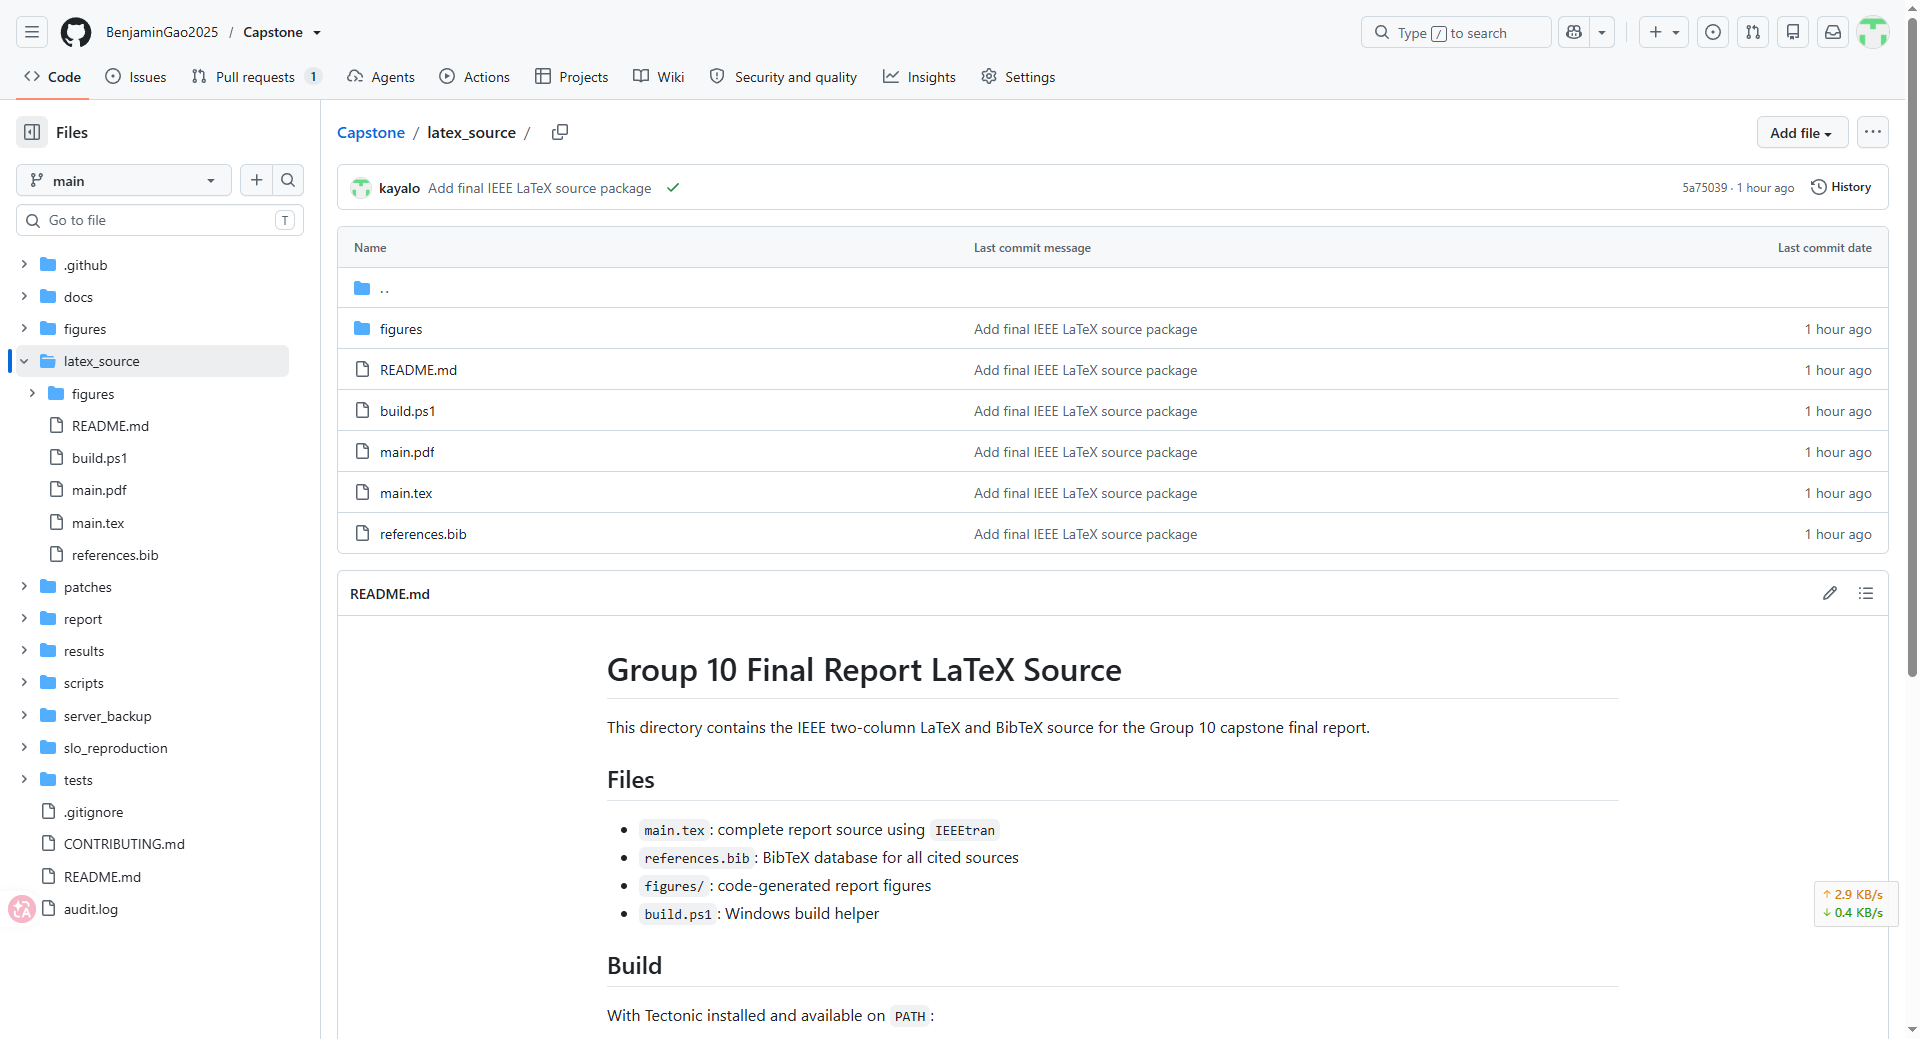
\includegraphics[width=0.94\textwidth]{figures/github_latex_source.png}
}{
    \fbox{\parbox[c][0.35\textheight][c]{0.86\textwidth}{
        \centering
        \textbf{FINAL INSERTION REQUIRED BEFORE PDF SUBMISSION}\\[1em]
        Replace this box with one real screenshot showing the top-level
        GitHub \texttt{latex\_source/} directory.
    }}
}
\caption{Top-level GitHub directory containing the final LaTeX and BibTeX source.}
\label{fig:github-source}
\end{figure}

\end{document}
